\ifx\wholebook\relax\else

% --------------------------------------------
% Lulu:

    \documentclass[a4paper,12pt,twoside]{../includes/ThesisStyle}

	\usepackage[T1]{fontenc} %%%key to get copy and paste for the code!
%\usepackage[utf8]{inputenc} %%% to support copy and paste with accents for frnehc stuff
\usepackage{times}
\usepackage{ifthen}
\usepackage{xspace}
\usepackage{alltt}
\usepackage{latexsym}
\usepackage{url}            
\usepackage{amssymb}
\usepackage{amsfonts}
\usepackage{amsmath}
\usepackage{stmaryrd}
\usepackage{enumerate}
\usepackage{cite}
%\usepackage[pdftex,colorlinks=true,pdfstartview=FitV,linkcolor=blue,citecolor=blue,urlcolor=blue]{hyperref}
\usepackage{xspace}
%\usepackage{graphicx}
\usepackage{subfigure}
\usepackage[scaled=0.85]{helvet}
        
        
\newcommand{\sepe}{\mbox{>>}}
\newcommand{\pack}[1]{\emph{#1}}
\newcommand{\ozo}{\textsc{oZone}\xspace}
\newcommand\currentissues{\par\smallskip\textbf{Current Issues -- }}

\newboolean{showcomments}
\setboolean{showcomments}{true}
\ifthenelse{\boolean{showcomments}}
  {\newcommand{\bnote}[2]{
	\fbox{\bfseries\sffamily\scriptsize#1}
    {\sf\small$\blacktriangleright$\textit{#2}$\blacktriangleleft$}
    % \marginpar{\fbox{\bfseries\sffamily#1}}
   }
   \newcommand{\cvsversion}{\emph{\scriptsize$-$Id: macros.tex,v 1.1.1.1 2007/02/28 13:43:36 bergel Exp $-$}}
  }
  {\newcommand{\bnote}[2]{}
   \newcommand{\cvsversion}{}
  } 


\newcommand{\here}{\bnote{***}{CONTINUE HERE}}
\newcommand{\nb}[1]{\bnote{NB}{#1}}
\newcommand{\fix}[1]{\bnote{FIX}{#1}}
%%%% add your own macros 

\newcommand{\sd}[1]{\bnote{Stef}{#1}}
\newcommand{\ja}[1]{\bnote{Jannik}{#1}}
\newcommand{\na}[1]{\bnote{Nico}{#1}}
%%% 


\newcommand{\figref}[1]{Figure~\ref{fig:#1}}
\newcommand{\figlabel}[1]{\label{fig:#1}}
\newcommand{\tabref}[1]{Table~\ref{tab:#1}}
\newcommand{\layout}[1]{#1}
\newcommand{\commented}[1]{}
\newcommand{\secref}[1]{Section \ref{sec:#1}}
\newcommand{\seclabel}[1]{\label{sec:#1}}

%\newcommand{\ct}[1]{\textsf{#1}}
\newcommand{\stCode}[1]{\textsf{#1}}
\newcommand{\stMethod}[1]{\textsf{#1}}
\newcommand{\sep}{\texttt{>>}\xspace}
\newcommand{\stAssoc}{\texttt{->}\xspace}

\newcommand{\stBar}{$\mid$}
\newcommand{\stSelector}{$\gg$}
\newcommand{\ret}{\^{}}
\newcommand{\msup}{$>$}
%\newcommand{\ret}{$\uparrow$\xspace}

\newcommand{\myparagraph}[1]{\noindent\textbf{#1.}}
\newcommand{\eg}{\emph{e.g.,}\xspace}
\newcommand{\ie}{\emph{i.e.,}\xspace}
\newcommand{\ct}[1]{{\textsf{#1}}\xspace}


\newenvironment{code}
    {\begin{alltt}\sffamily}
    {\end{alltt}\normalsize}

\newcommand{\defaultScale}{0.55}
\newcommand{\pic}[3]{
   \begin{figure}[h]
   \begin{center}
   \includegraphics[scale=\defaultScale]{#1}
   \caption{#2}
   \label{#3}
   \end{center}
   \end{figure}
}

\newcommand{\twocolumnpic}[3]{
   \begin{figure*}[!ht]
   \begin{center}
   \includegraphics[scale=\defaultScale]{#1}
   \caption{#2}
   \label{#3}
   \end{center}
   \end{figure*}}

\newcommand{\infe}{$<$}
\newcommand{\supe}{$\rightarrow$\xspace}
\newcommand{\di}{$\gg$\xspace}
\newcommand{\adhoc}{\textit{ad-hoc}\xspace}

\usepackage{url}            
\makeatletter
\def\url@leostyle{%
  \@ifundefined{selectfont}{\def\UrlFont{\sf}}{\def\UrlFont{\small\sffamily}}}
\makeatother
% Now actually use the newly defined style.
\urlstyle{leo}



	\usepackage{amsmath,amssymb}             % AMS Math
% \usepackage[french]{babel}
\usepackage[latin1]{inputenc}
\usepackage[T1]{fontenc}
\usepackage[left=1.5in,right=1.3in,top=1.1in,bottom=1.1in,includefoot,includehead,headheight=13.6pt]{geometry}
\renewcommand{\baselinestretch}{1.05}

\usepackage{multicol}

% Table of contents for each chapter

\usepackage[nottoc, notlof, notlot]{tocbibind}
\usepackage{minitoc}
\setcounter{minitocdepth}{1}
\mtcindent=15pt
% Use \minitoc where to put a table of contents

\usepackage{enumitem}

\usepackage{aecompl}

% Glossary / list of abbreviations

%\usepackage[intoc]{nomencl}
%\renewcommand{\nomname}{List of Abbreviations}
%
%\makenomenclature

% My pdf code

\usepackage[pdftex]{graphicx}
\usepackage[a4paper,pagebackref,hyperindex=true]{hyperref}

\usepackage{pgfplotstable,booktabs,colortbl}
\pgfplotsset{compat=1.8}

% Links in pdf
\usepackage{color}
\definecolor{linkcol}{rgb}{0,0,0.4} 
\definecolor{citecol}{rgb}{0.5,0,0} 

% Change this to change the informations included in the pdf file

% See hyperref documentation for information on those parameters

\hypersetup
{
bookmarksopen=true,
pdftitle="Sista: a Metacircular Architecture for Runtime Optimisation Persistence",
pdfauthor="Clement BERA", 
pdfsubject="Thesis", %subject of the document
%pdftoolbar=false, % toolbar hidden
pdfmenubar=true, %menubar shown
pdfhighlight=/O, %effect of clicking on a link
colorlinks=true, %couleurs sur les liens hypertextes
pdfpagemode=None, %aucun mode de page
pdfpagelayout=SinglePage, %ouverture en simple page
pdffitwindow=true, %pages ouvertes entierement dans toute la fenetre
linkcolor=linkcol, %couleur des liens hypertextes internes
citecolor=citecol, %couleur des liens pour les citations
urlcolor=linkcol %couleur des liens pour les url
}

% definitions.
% -------------------

\setcounter{secnumdepth}{3}
\setcounter{tocdepth}{1}

% Some useful commands and shortcut for maths:  partial derivative and stuff

\newcommand{\pd}[2]{\frac{\partial #1}{\partial #2}}
\def\abs{\operatorname{abs}}
\def\argmax{\operatornamewithlimits{arg\,max}}
\def\argmin{\operatornamewithlimits{arg\,min}}
\def\diag{\operatorname{Diag}}
\newcommand{\eqRef}[1]{(\ref{#1})}

\usepackage{rotating}                    % Sideways of figures & tables
%\usepackage{bibunits}
%\usepackage[sectionbib]{chapterbib}          % Cross-reference package (Natural BiB)
%\usepackage{natbib}                  % Put References at the end of each chapter
                                         % Do not put 'sectionbib' option here.
                                         % Sectionbib option in 'natbib' will do.
\usepackage{fancyhdr}                    % Fancy Header and Footer

% \usepackage{txfonts}                     % Public Times New Roman text & math font
  
%%% Fancy Header %%%%%%%%%%%%%%%%%%%%%%%%%%%%%%%%%%%%%%%%%%%%%%%%%%%%%%%%%%%%%%%%%%
% Fancy Header Style Options

\pagestyle{fancy}                       % Sets fancy header and footer
\fancyfoot{}                            % Delete current footer settings

%\renewcommand{\chaptermark}[1]{         % Lower Case Chapter marker style
%  \markboth{\chaptername\ \thechapter.\ #1}}{}} %

%\renewcommand{\sectionmark}[1]{         % Lower case Section marker style
%  \markright{\thesection.\ #1}}         %

\fancyhead[LE,RO]{\bfseries\thepage}    % Page number (boldface) in left on even
% pages and right on odd pages
\fancyhead[RE]{\bfseries\nouppercase{\leftmark}}      % Chapter in the right on even pages
\fancyhead[LO]{\bfseries\nouppercase{\rightmark}}     % Section in the left on odd pages

\let\headruleORIG\headrule
\renewcommand{\headrule}{\color{black} \headruleORIG}
\renewcommand{\headrulewidth}{1.0pt}
\usepackage{colortbl}
\arrayrulecolor{black}

\fancypagestyle{plain}{
  \fancyhead{}
  \fancyfoot{}
  \renewcommand{\headrulewidth}{0pt}
}

\usepackage{algorithm}
\usepackage[noend]{algorithmic}

%%% Clear Header %%%%%%%%%%%%%%%%%%%%%%%%%%%%%%%%%%%%%%%%%%%%%%%%%%%%%%%%%%%%%%%%%%
% Clear Header Style on the Last Empty Odd pages
\makeatletter

\def\cleardoublepage{\clearpage\if@twoside \ifodd\c@page\else%
  \hbox{}%
  \thispagestyle{empty}%              % Empty header styles
  \newpage%
  \if@twocolumn\hbox{}\newpage\fi\fi\fi}

\makeatother
 
%%%%%%%%%%%%%%%%%%%%%%%%%%%%%%%%%%%%%%%%%%%%%%%%%%%%%%%%%%%%%%%%%%%%%%%%%%%%%%% 
% Prints your review date and 'Draft Version' (From Josullvn, CS, CMU)
\newcommand{\reviewtimetoday}[2]{\special{!userdict begin
    /bop-hook{gsave 20 710 translate 45 rotate 0.8 setgray
      /Times-Roman findfont 12 scalefont setfont 0 0   moveto (#1) show
      0 -12 moveto (#2) show grestore}def end}}
% You can turn on or off this option.
% \reviewtimetoday{\today}{Draft Version}
%%%%%%%%%%%%%%%%%%%%%%%%%%%%%%%%%%%%%%%%%%%%%%%%%%%%%%%%%%%%%%%%%%%%%%%%%%%%%%% 

\newenvironment{maxime}[1]
{
\vspace*{0cm}
\hfill
\begin{minipage}{0.5\textwidth}%
%\rule[0.5ex]{\textwidth}{0.1mm}\\%
\hrulefill $\:$ {\bf #1}\\
%\vspace*{-0.25cm}
\it 
}%
{%

\hrulefill
\vspace*{0.5cm}%
\end{minipage}
}

\let\minitocORIG\minitoc
\renewcommand{\minitoc}{\minitocORIG \vspace{1.5em}}

\usepackage{multirow}
\usepackage{slashbox}

\newenvironment{bulletList}%
{ \begin{list}%
	{$\bullet$}%
	{\setlength{\labelwidth}{25pt}%
	 \setlength{\leftmargin}{30pt}%
	 \setlength{\itemsep}{\parsep}}}%
{ \end{list} }

\newtheorem{definition}{D�finition}
\renewcommand{\epsilon}{\varepsilon}

% centered page environment

\newenvironment{vcenterpage}
{\newpage\vspace*{\fill}\thispagestyle{empty}\renewcommand{\headrulewidth}{0pt}}
{\vspace*{\fill}}



	\graphicspath{{.}{../figures/}}
	\begin{document}
\fi

\chapter{Metacircular optimiser and deoptimiser}
\label{chap:metacircular}
\minitoc

%Intro
By design, the runtime optimiser and deoptimiser are written in Smalltalk and are running in the same runtime than the optimised application. This design leads to multiple problems similar to problems existing in metacircular virtual machine. 

%single-threaded -> for comparison with Graal and co later
As Pharo is currently single-threaded, it is not possible to run Scorch in a concurrent native thread. To optimise code, Scorch requires either to interrupt the application green thread temporarily or to postpone the optimisation to a background-priority green thread. The deoptimiser cannot however postpone its tasks as it would block completely the running application, hence it has to interrupt the application green thread until the deoptimisation is done.

%introduction of the main issue
We call the \emph{infinite recursion} problem the main issue. The infinite recursion happens in both the optimiser and the deoptimiser. When a frequent portion of code is detected in the optimiser code, it interrupts itself and starts to optimise one of its own v-function. While doing so, the same frequent portion of code is detected and the optimiser interrupts itself again to optimise the same v-function, until it interrupts itself again, completely freezing the application. When the deoptimiser requires to deoptimise a function to be able to keep deoptimising an optimised frame, it calls itself, which may require to deoptimise the same function, leading to the deoptimiser calling itself again and again, also completely freezing the application.

%Different constraint so different solutions
The optimiser and deoptimiser have different constraints. For example, it is possible to disable temporarily the optimiser, which in the worst case leads to some functions not to be optimised, but it is not possible to disable temporarily the deoptimiser as it is required to execute code. As they have different constraints, they need different solutions for the infinite recursion problem. In both cases, the management of the dependencies of the framework is critical to ensure that the infinite recursion issue is solved.

%Outline and solution
This chapter explains the design used to avoid the infinite recursion issue in both the deoptimiser and the deoptimiser. For each of them, we specify what constraints we enforce on package dependencies and on the runtime to make sure the problem is entirely solved. The problem is solved in the optimiser by defining a critical portion of code in the optimiser where it disables itself temporarily, ensuring that it cannot be triggered on this part of its own code. The deoptimiser solves the problem by using code completely independent from the rest of the system that cannot be optimised, hence never requires to be deoptimised. The last section discuss similar design issues in other VMs and when relevant, compares our solution to other solutions.

%%%%%%%%%%%%%%%%%%%%%%%%%%%%%%%%%%%%%%%%%%%%%%%%%%%%%%%%%%%%%%%%%%%%%%%%%%%%%%%%%%%%%%%%%%%%%%%%%%%%%%%%%%%%%%%%%%%%%%%%%%%%%

\section{Scorch optimiser}

%Intro
Cogit was extended to detect frequently used portion of code based on profiling counters. When such a portion of code is detected, Cogit triggers a call-back to request Scorch to optimise a v-function based on the current state. The overall design is then the following: the optimiser interrupts temporarily the application green thread, finds a v-function to optimise based on the current stack, optimises and installs the optimised version, then resumes the application. The optimised v-function installed will be executed at the next call of the function.

\subsection{Optimiser critical and background modes}

%TimeBeforePostPoning: problem so it's required
This design is too naive because the optimiser may interrupt the application for a long time. Indeed, optimising a function can take a long time in slow machines or when a pathological function is optimised. To experiment with the optimiser, we worked mainly using one application, the development environment of Pharo. In the case of a user-interface application, it is \emph{very} annoying to see the application interrupted during half a second or more, it feels like the user interface is slow, lagging and unresponsive.

%First solution: timeBeforePostponing, with constraint for long methods
To avoid the problem, we limited the time window of the optimiser to a small amount of time, configurable from the language. For the development tools, we limited it to 40 ms. The limitation is enforced by a high-priority green thread, set to stop the optimiser after a given amount of time. As the current tools are refreshing at 50Hz, it means that the optimiser, at worst, force the system to drop two frames. In practice, most v-functions are optimised in less than 40ms. However, we now have a significant problem: v-functions too long to optimise are not optimised at all.

%idle and postpone
Upon profiling, we noticed, as expected, that this user interface application spends a significant amount of time in idle\footnote{An application in idle means it has nothing to do, it is typically waiting for an event to do anything.}. We show for example in figure \ref{fig:ApplicationIdle} that the application is successfully executing code, then idle, then executing code again, etc. 

\begin{figure}[h!]
    \begin{center}
        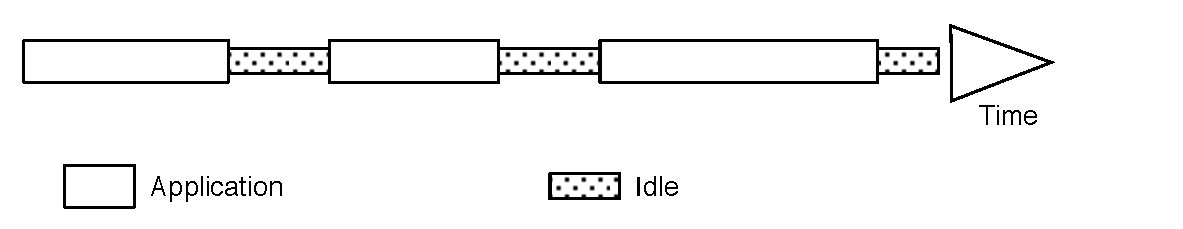
\includegraphics[width=0.9\linewidth]{ApplicationIdle}
        \caption{User interface application idle times}
        \label{fig:ApplicationIdle}
    \end{center}
\end{figure}

%background thread
Based on this result, we introduced a background green thread responsible for optimising the v-function too long to optimise in the small time window. Hence, when the application would normally become idle, it starts by optimising such v-functions until and becomes idle when no v-functions to optimise are remaining.

\begin{figure}[h!]
    \begin{center}
        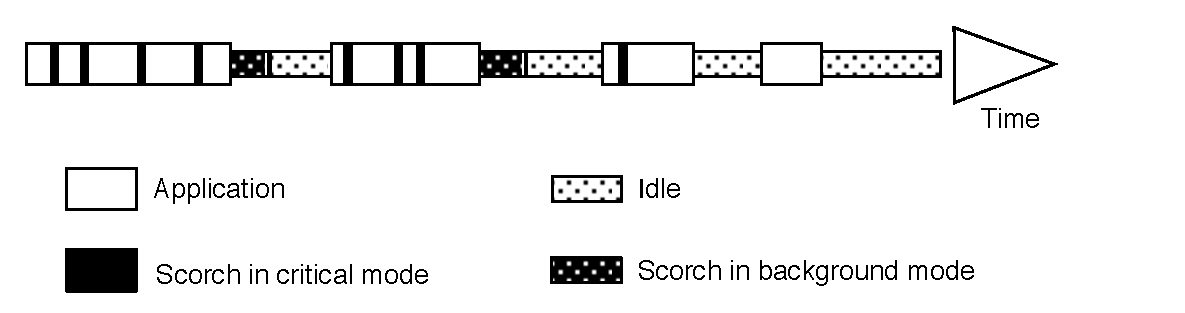
\includegraphics[width=0.9\linewidth]{ScorchModes}
        \caption{Scorch critical and background modes}
        \label{fig:ScorchModes}
    \end{center}
\end{figure}

%Fig explanation, critical vs background mode
As shown on figure \ref{fig:ScorchModes}, when the application is running, it can be interrupted for a small time window at worst. When the application normally becomes idle, the background green thread starts optimising the v-functions long to optimise. When no more v-functions are queued for optimisations, the application becomes idle. In any case, after a while, all critical portion of code have been optimised and the application is usually not interrupted any more while the background green thread has usually no more v-functions to optimise.

\paragraph{Conclusion.} The Scorch optimiser can be run in two modes. On critical mode, it interrupts the application green thread and has a limited time-window to optimise a function. On background mode, it optimises code only when the application is idle but as no time limit. 

\subsection{Infinite recursion}

%repeat problem for optimiser
As Scorch is written in Smalltalk, it can theoretically optimise its own code. In practice, if Scorch is triggered on itself, it may lead to an infinite recursion. Indeed, each time Scorch tries to optimise anything, before reaching the point where it can install the optimised function, it may interrupt itself to start optimising one of its own function. If a frequent portion of code is detected at each optimisation attempt, then Scorch never reaches the point where it can install optimised function because it keeps restarting new optimisation on its own code.

%slow down - nothing happen in critical and slow but succeed in background mode
In critical mode, Scorch has a limited time window. Hence, if the infinite recursion happens, the optimiser gets stuck until the time window ends, then the application resumes without any optimised function installed. In background mode, the optimisation is slower because the optimiser gets stuck in critical mode multiple times, but at some point the code gets optimised and installed.

\paragraph{First solution.} The first solution we thought of is to disable to optimiser when it is running. We believed it would solve the problem at the cost that the optimiser would not be able to optimise itself, and we were willing to to accept this consequence.

%Optimiser can be disabled
The optimiser is considered disabled when each call-back normally starting the optimisation of code is modified not to do anything at all. In this case, the application keeps running, using non optimised code or code optimised when the optimiser was enabled.

%call-back removal / addition implementation
To implement our first solution, we changed the VM call-back activating the optimiser to uninstall itself upon activation. Then, we changed the optimiser so that when it resumes the application, after postponing the optimisation or installing optimised code, it installs back the call-back. This way, we thought the optimiser would never end up in a situation where it optimises itself, solving entirely the problem.

%can optimise itself through back process
Then, we run our benchmarks and see that the problem was solved but the optimiser could still optimise its own code. Our implementation effectively disabled the optimiser, but only while it was on critical mode. Hence, when frequent portions of code of the application were detected, they were optimised or postponed without any issue as the optimiser disabled itself during this phasis, and the application resumed just fine. However, when the optimiser was run in background mode, it was not disabled. Hence, in this case, the optimiser in background was sometimes interrupted by itself in critical mode to get optimised.

\paragraph{Discussion and future solutions}

%1st sol work and good enough 
The first solution is implemented and works fine. The application runs with significant speed-up over the normal VM. In general, in the production VM, simplicity is really important to keep the code relatively easily maintanable and for each added complexity in the VM we wonder if the complexity is worth the benefit. The first solution is satisfying enough and we may move to production with this solution.

%but cannot optimise itself in critical mode
Now, there is still one minor design issue: the optimiser cannot optimise itself in critical mode. Even worse, as the profiling counters are encoded in 16 bits, if one of them exceeds 65535 on one of the optimiser method in critical mode, the counters are reset and the frequently portion of code is not detected at all.

%the postpone pb while in critical mode
Based on advises from other VM developer, we considered, instead of disabling the optimiser when it is running in critical mode, to postpone the optimisation to the background mode. In our design, it is quite difficult to do so. Indeed, when the VM call-back starts the optimiser, it provides a reification of the current stack. The optimiser then needs to scan the stack to select what function it should optimise. 


[ BEGIN TO CHECK: the following few paragraph on stack search may belong to another chapter.

%Function selection ->maybe move to another section ?
In most cases, the optimiser does not pick the function of the bottom stack frame to perform optimisations. The reason is because an important part of the performance overhead in Smalltalk comes from the extensive use of closures. Especially, most loops in the executed code, assuming they respect standard Smalltalk coding conventions, are using closures. To efficiently remove the closure overhead, the closure needs to be inlined up to its enclosing environment. Hence, the optimiser usually picks the function where closures are created. 

\paragraph{Loop example.} To illustrate the closure issue and why the optimiser usually picks another function than the bottom frame's function, we will use an example with a loop over an array. 

%array loop example. descr exampleArrayLoop
In the code sample shown below, \ct{exampleArrayLoop} is a method installed in the class \ct{ApplicationClass}. Its method body consists of a loop over an array, the array being an instance variable. To loop over an array, Smalltalk provides high level construct such as \ct{do:}. In this case, \ct{do:} is very similar to \ct{foreach} in other languages and allows to iterate over the array while providing at each iteration of the loop the array's element in the variable \ct{element}. The \ct{do:} method takes a single argument, a closure, which is evaluated using \ct{value:} at each iteration of the loop.

\begin{code}
	ApplicationClass >> exampleArrayLoop
	    array do: [ :element | FileStream stdout nextPutAll: element printString ].
		
	Array >> do: aBlock
	    1 to: self size do: [:index | aBlock value: (self at: index)].
\end{code}

%descr do:
The method \ct{Array >> do:} is using a special selector, \ct{to:do:}, which is compiled by the bytecode compiler to a loop, in a similar way to \ct{for} constructs in other languages. In fact, this method is a loop from 1 to the size of the array. Index starts with the value 1 and is incremented by 1 at each iteration of the loop. At each iteration, the current value of index is tested against the size of the array, and when that value is reached the loop is exited.

%profiling counter location
As discussed before, profiling counters detect frequent portion of code on branches. Each finite loop has a branch to either keep iterating over the loop or exit the loop. In the example, it means that the method \ct{Array >> do:} has a profiling counter on the branch testing the value of the index against the size of the array. The rest of the code, in the two methods and in the closure, have no other profiling counters, though they may call functions having other profiling counters.

%closure issue and why to pick next function
A frequent portion of code is going to be detected on the profiling counter, hence in the method \ct{Array >> do:}. The main issue is that an important part of the execution time is spent both in creating and evaluating the closure, and from the \ct{Array>>do:} method, it is not possible to knwo what closure will be executed. Hence, the optimiser is likely to decide to optimise \ct{ApplicationClass >> exampleArrayLoop} so it will be able to inline \ct{Array >> do:}, and then the closure evaluation (\ct{value:}), completely removing the need for the closure hence removing its allocation.

%closure last explanation
Overall, because of the extensive use of closures, the optimiser usually never pick the bottom stack frame function for optimisation. It usually walk up a few frames to find the best function to optimise. 

END TO CHECK ]


%current point.
As the current stack is modified upon execution, it is not possible to save it efficiently so that the optimiser can look at it in the background green thread. It is possible, however, once the optimiser has found what function to optimise, to keep a list of such functions and postpone their optimisation. We therefore believe that instead of disabling the optimiser while it is running in critical mode, we could instead disable it only during the stack scanning phase in critical mode, which represent less than 1\% of execution time, and postpone the optimisation to the background green thread. Hence only the code of this part of the optimiser could not be optimised in critical mode. The rest of the optimiser would be optimised at the first long enough idle pause.

\paragraph{Preheating and static compilation.} As the Sista architecture allows to persist optimise code, the optimiser's code could be preheated through warm-up runs, for example by giving it a list of well-chosen functions to optimise. This way, all frequent portions of code would be detected ahead of time and optimised before shipping the runtime to production. If warm-ups are too unreliable, alternatively, the optimiser could be optimised statically by calling itself on its own code, using types infered from a static type inferencer instead of types providing by the runtime application. This last alternative comes with all the advantages and problems of static ahead-of-time compilation.


\subsection{Dependencies and optimisations} 

% from 1 old part
%Rephrase -  solution does not forbig Scorch to use optimise libs
The flag approach has a significant advantage: it is quite simple both conceptually and implementation-wise, while it completely avoids the infinite recursion problem. It has however a major drawback: Scorch cannot optimise its own code any more. Of course, Scorch uses core libraries that can be optimised. The main case are the core collections, if the application optimised is also using core collections, they may get optimised, then Scorch ends up using an optimised collection library. For this reason, it is possible that while optimising code Scorch triggers the deoptimiser, and it works perfectly fine.

% maybe only one sentence ? -> be careful about dependencies
The first constraint to note when programming Scorch, which may be obvious to the Kernel programmer, is that Scorch cannot depends on any framework or library but the Kernel and Core libraries. Each framework or library in the system relies on the execution engine to perform its code. Scorch is part of the execution engine. Hence, if Scorch relies on an external library and that someone modifies the library, the execution engine may not be stable any more and the runtime completely crashes. In fact, all the Kernel code and Core librairies have similar constraints, they cannot rely on anything to keep the system modular. 
-
While writting Scorch, we needed a tool to compress the deoptimisation metadata generated aside from the optimised code. We wanted to use the standard Pharo serializer, Fuel (CITE), but we were not able to do it or further modification on Fuel would break the execution engine.
-
In the end, we limited the dependencies of Scorch to the Pharo Kernel and the core collections (exactly: Set, OrderedCollection, Array, ByteArray and Dictionary in addition to the kernel). Any change on one of this dependency may require to change something in Scorch to keep the system running.


%\subsection{Debugging and runtime modification}

%Should I talk about that at all ? I was thinking over a restricted compiling to C but maybe we don't care.

%Maybe rewrite so that formally does not work but in practice it does.

%As any Smalltalk program, it is possible to modify the optimiser while it is running, for example in the debugger. If the modifications leads to incorrect optimiser behavior, then the runtime may crash. To avoid crashes, it may be wise to disable the optimiser while editing it. In practice, this feature is used only by the optimiser implementors. It is very useful to debug the optimiser to understand specific bugs or compiler decisions. With careful understanding of the infrastructure, it is possible in practice to debug the optimiser while it is running and modify its code. The optimiser is set by default to catch all exceptions, failing the optimisation of a specific v-function if an exception was raised. Hence, if the code modification triggers a compile-time exception, the system shall not crash. Unfortunately, in some cases, the optimiser may have silent errors, generating incorrect code without raising exceptions and completely crashing the system.

%The only part of Scorch that cannot really be edited is the deoptimisation metadata generation. Indeed, deoptimisation metadata is also used by the deoptimiser which, as detailled in the following section, has stronger constraints on its code. If one modifies the deoptimisation metadata generated, the deoptimiser may not be able to deoptimise correctly optimised code any more, leading to crashes.




%%%%%%%%%%%%%%%%%%%%%%%%%%%%%%%%%%%%%%%%%%%%%%%%%%%%%%%%%%%%%%%%%%%%%%%%%%%%%%%%%%%%%%%%%%%%%%%%%%%%%%%%%%%%%%%%%%%%%%%%%%%%%

\section{In-language deoptimiser}

The trap instruction is present in the extended bytecode set and when reached through execution flow, Cogit triggers a call-back to the deoptimiser. In addition, multiple tools in the language, such as the debugging tools, have been changed to call the deoptimiser when the programmer attempts to introspect the stack.

On the contrary to the optimiser, deoptimisation cannot be postponed to a background green thread, or the application green thread may be blocked until the application reaches idle state. In addition, deoptimisation cannot fail or the runtime crashes. If the optimiser failed to create an optimised function, then the execution could simply fall back to non optimised code. If the deoptimiser fails to recreate a non optimised version of the stack, then the system crashes or the application green thread has to be terminated.

%TODO I think I mean it cannot be disabled.

As the deoptimiser cannot fail, it is not possible to solve the infinite recursion problem in the same way than the optimiser. If the deoptimiser request deoptimisation, as for the optimiser requesting optimisation, the programs ends up in an infinite recursion where it keeps deoptimising / optimising itself. In the case of the optimiser, we could simply disable it while it is running, and the entire problem was solved. In the case of the deoptimiser, if we disable it and the deoptimiser request deoptimisation, the program cannot resume using non optimised code and crashes. 

To solve this infinite recursion problem, we implemented two solutions. The first solution attempts to restore the system in a recovery mode when recursive deoptimisation happens. It was used for the first benchmark, but it did not work correctly with benchmarks creating multiple green threads, and making it thread-safe had too many constraints. Then a second solution, used now, was designed and consists in keeping all the deoptimiser code in a library completely independent from the rest of the system that cannot be optimised.

\subsection{Recovery mode}

In this first solution to the infinite recursion problem for deoptimisation, we attempted to keep a recovery state of the whole system. More precisely, Scorch kept a copy of the method dictionaries

 Attempt to recovery state with limited portion that cannot be optimised, issues with green threads and complexity, made it independent.

cannot optimie until flag set / reset.

- recovery state (not working with threads)

too difficult to make thread safe because then up until the flag is set we could not optimise hence can't optimise code in process scheduler.

\subsection{Independent library}

- completely independent and forbid deopt / opt

We could opt it statically.

Strong constraints: no dependency at all (duplicate array and dict), debugging is hardly possible.

Example of debugging -> can't log from deoptimiser. 

\subsection{Debugging and runtime modification}

Modifying the deoptimiser while it is running is also more complex than the optimiser. Optimised code is present in the runtime, and any modification of the deoptimiser is

- any change imply existing code cannot be deopt and hard crashes.

%%%%%%%%%%%%%%%%%%%%%%%%%%%%%%%%%%%%%%%%%%%%%%%%%%%%%%%%%%%%%%%%%%%%%%%%%%%%%%%%%%%%%%%%%%%%%%%%%%%%%%%%%%%%%%%%%%%%%%%%%%%%%

\section{Related work}

\subsection{DSL compiled to machine code}

Modification at runtime of the optimiser in our case (Smalltalk + same runtime), though crashes.
Restrictive.

\subsection{Metacircular VMs}

In general this problem is solved, for example with magic or threads (Jalapeno).

\subsection{Graal}

Stack search and deoptimisation in the VM


In chapter \ref{chap:stateOfTheArt}, we introduced multiple metacircular VMs. 


%%%%%%%%%%%%%%%%%%%%%%%%%%%%%%%%%%%%%%%%%%%%%%%%%%%%%%%%%%%%%%%%%%%%%%%%%%%%%%%%%%%%%%%%%%%%%%%%%%%%%%%%%%%%%%%%%%%%%%%%%%%%%

\section{Conclusion}

In this chapter we discussed the main issues existing because the optimiser and the deoptimiser are implemented in Smalltalk and are running in the same runtime and the same native thread than the application they optimise and deoptimise respectively. The main issues are related to infinite recursion. If a frequently used portion of code is detected inside the optimiser code, the optimiser may call itself indefinitely by trying to optimise the portion of code, and while doing so, calling itself. The deoptimiser has the same issue when it needs to deoptimise its own code. In both cases, the program may get stuck.

The optimiser solves this issue by disabling itself when it runs by interrupting the application green thread. In most case, this means that the optimiser cannot optimise its own code. In practice, v-functions too long to optimise within a small time window are postponed in a background green thread, running when the application is in idle. When the optimiser is started through the background green thread, it can optimise itself.

The deoptimiser cannot solve the problem the same way.

 to optimise may  or if the deoptimiser calls itself to deoptimise its code, the program may get stuck. As an optimisation can be cancelled, the optimiser can simply be disabled while it is optimising something. 

%repeat again.

\ifx\wholebook\relax\else
    \end{document}
\fi